%%%%%%%%%%%%%%%%%%%%%%%%%%%%%%%%%%%%%%%%%%%%%%%%%%%%%%%%%%%%%%%%%%%
%\begin{bibunit}[apalike]
\begin{frame}%[label=frm:20]
	\frametitle{Trabajo Actual \cite{hutzenthaler2015numerical}}
		\begin{overlayarea}{\linewidth}{.3\textheight}
			\only<2>{
				\begin{empheq}[box=\shadowbox*]{align*}
					dy_1(t) &=
						y_1(t) \left[1 - y_1(t) + 2 y_2(t) \right]dt + \varepsilon y_1^2(t) dW_1(t), \\
					dy_2(t) &=
						y_2(t) \left[1 - 2 y_2(t) + 2 y_1(t)\right]dt + \varepsilon y_2^2(t) dW_2(t).
				\end{empheq}
		}
		\only<3>{
			\vspace{-.5cm}
			\begin{empheq}[]{align*}
				dy_1(t) &=
				\left(
				\lambda -\delta y_1(t) - (1 - \gamma) \beta y_1(t) y_3(t)
				\right)dt,
				-\sigma_1 y_1(t) dW^{(1)}_t, 
				\notag \\
				dy_2(t) &= 
				\left(
				(1- \gamma) \beta y_1(t) y_3(t) - a y_2(t) 
				\right)dt,
				-\sigma_1 y_2(t) dW^{(1)}_t, 
				\\
				dy_3(t) & = 
				\left(
				(1 - \eta) N a y_2(t) 
				-u y_3(t)
				-(1 - \gamma ) \beta y_1(t) y_3(t) 
				\right)dt
				- \sigma_2 y_3(t) dW^{(2)}_t.
				\notag
				\end{empheq}
		}
		\only<4>{
			\begin{empheq}[box=\shadowbox]{equation*}
				dX_t=- X_t^5 dt + X_tdW_t, \qquad X_0=1
			\end{empheq}
			}
		\only<5>{
			\begin{empheq}[box=\shadowbox]{align*}
				dy(t)&= \left[by(t)-a y(t)^2\right]dt + \sigma y(t) dW_t,\\
				y(t)&= \frac{
						y_0
						\exp\left[
						b-\frac{1}{2}\sigma^2) t
						+\sigma W_t
						\right]
					}{
					1+a 
					y_0
					\int_0^t
					\exp\left[
					(b -\frac{1}{2})s
					+\sigma W_s
					\right]ds
						}
			\end{empheq}
		}
		\only<6>{
			\begin{empheq}[box=\shadowbox]{align*}
				dX_t^{(1)}&= X_t^{(2)} dt\\
				dX_t^2&=\left\{
				\mu X_t^{(2)}(1 -(X_t^{(1)})^2)-X_t^{1}
				\right\}dt
				+\sigma dW_t
			\end{empheq}
			}
			\only<7>{
				\vspace{-.3cm}
				\begin{empheq}[box=\shadowbox]{equation*}
					dy(t) = -y^3 dt 
					+ \frac{1}{\left[\log(t+1)\right]^{1.1}} dW_t, \qquad t>0.
				\end{empheq}
		}
		\end{overlayarea}
%	
%	
%	
	\begin{overlayarea}{\linewidth}{.8\textheight}
		\only<2>{
			\includegraphics[width=0.5\linewidth]{images/StoDetX1Mao.png}
			\includegraphics[width=0.5\linewidth]{images/StoDetX2Mao.png}
		}
		\only<3>{
			\begin{center}
				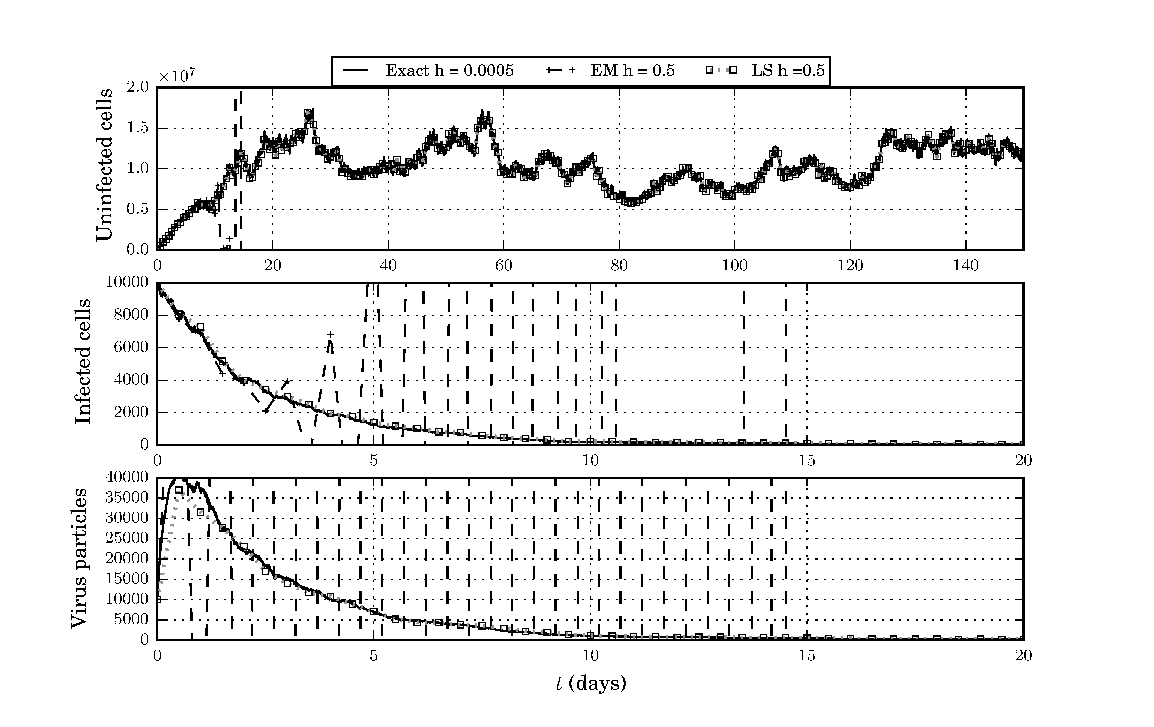
\includegraphics[width=0.8\linewidth]{images/InternalHIVDynamics5e-1}
			\end{center}
		}
		\only<4>{
			\begin{center}
				\includegraphics[width=0.7\linewidth]{images/MSETime2}
			\end{center}
		}
		\only<5>{
			\begin{center}
				\includegraphics[width=0.7\linewidth]{images/PathsLVEv4}
			\end{center}
		}
		\only<6>{
			\begin{center}
				\includegraphics[width=0.3\linewidth]{images/PhasePotraitSimDuffingVanDerPol.png}
				\includegraphics[width=0.3\linewidth]{images/X1SimDuffingVanDerPol}
				\includegraphics[width=0.3\linewidth]{images/X2SimDuffingVanDerPol}
			\end{center}
		}
		\only<7>{
			\vspace{-1.1cm}
			\begin{center}
				\includegraphics[width=0.45\linewidth]{images/pathsAppleby2}
			\end{center}
		}
	\end{overlayarea}
\end{frame}
%\end{bibunit}
%%%%%%%%%%%%%%%%%%%%%%%%%%%%%%%%%%%%%%%%%%%%%%%%%%%%%%%%%%%%%%%%%%%